\documentclass{article}

\usepackage{framed}
\usepackage[margin=2.5cm]{geometry}
\usepackage{graphicx}
\usepackage{hyperref}
\usepackage{tikz}
\usetikzlibrary{fit}

\renewcommand{\familydefault}{\sfdefault}

\setlength{\tabcolsep}{20pt}
\renewcommand{\arraystretch}{2}

\newcommand{\fignote}[1]{{\small{#1}}}

\title{A gentle introduction to data visualization in R for TAP Striking
  Statistics}
\date{March 2020}

\begin{document}
\maketitle

\section{Goals of this tutorial}

It is often easier and quicker to communicate coding concepts
    in an interactive in-person workshop. We are unlikely to have that
    opportunity soon. The idea of this tutorial is to have some
    self-guided examples, followed by a virtual Q\&A session
 
I have selected resources and examples with two goals in mind:
\begin{enumerate}
\item You can explore examples with enough background information to
  get a fair feel for the possibilities and challenges of data
  visualization in R
  \item We have enough of a shared understanding to jointly edit the
    occasional visualation, even if we use mostly use different
    tools

    \begin{framed}
    For example, a few weeks ago we needed to change a couple
    of maps to represent Western Sahara. Alexis had the correct
    shapefiles; Hannah and I had two different maps produced with two
    different workflows. If we had been a bit more coordinated,
    changing the underlying maps would have involved one line of reproducible
    code. (See example \ref{tap_map}). As it was, Hannah and I painted
    over our existing maps in Microsoft Paint.
  \end{framed}
\end{enumerate}
    
  \textbf{This is not}
\begin{itemize}
\item  A comprehensive introduction to R, to
      data visualization or even to data visualization in R
\item (Yet {\tt:-)}) An evangelistic mission to convert everyone to R
  
\end{itemize}


\section{Why R for data visualization?}

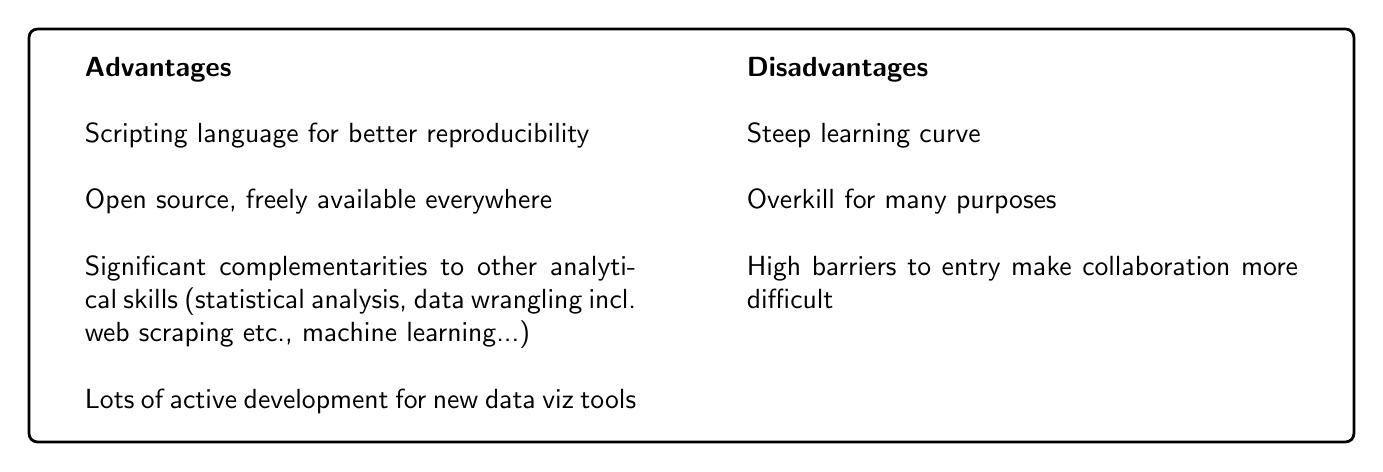
\begin{tikzpicture}
 \node[inner sep=0pt] (tab){%
\begin{tabular}[hbt]{p{7cm}p{7cm}}

  \textbf{Advantages} & \textbf{Disadvantages} \\
  Scripting language for better reproducibility & Steep
                                                               learning
                             curve\\
  Open source, freely available everywhere & Overkill for many
                                             purposes\\
  
  Significant complementarities to other analytical skills
  (statistical analysis, data wrangling incl. web scraping etc.,
  machine learning...)&High barriers to entry make collaboration more difficult\\
  Lots of active development for new data viz tools &\\

\end{tabular}
};
\node[draw=black, inner sep=0pt, rounded corners=3pt, line width=1pt,
fit=(tab.north west) (tab.north east) (tab.south east) (tab.south west)] {};
\end{tikzpicture}

\vspace{2em}

\textbf{Who else is using R?} https://github.com/ThinkR-open/companies-using-r


\begin{figure}
  \caption{Jobs and scholarly articles using different programming
    languages in 2018}
  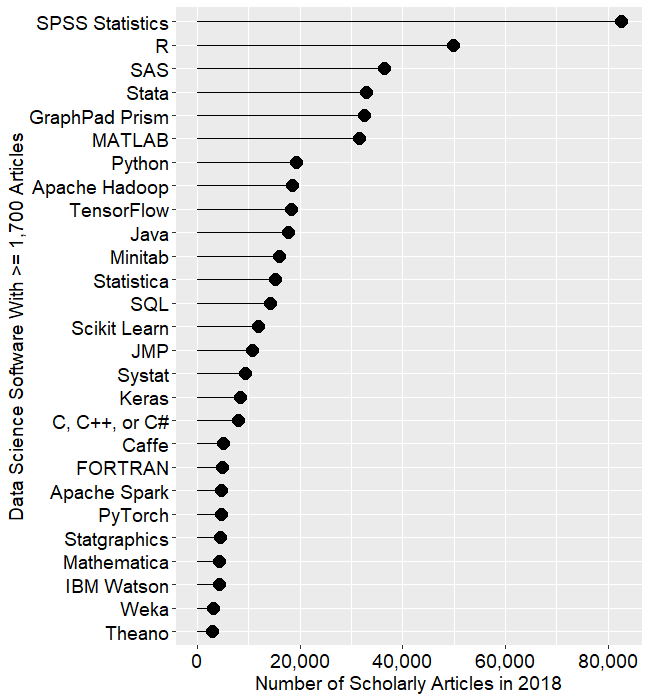
\includegraphics[width =  0.47\textwidth]{pictures/number_of_scholarly_articles}%
  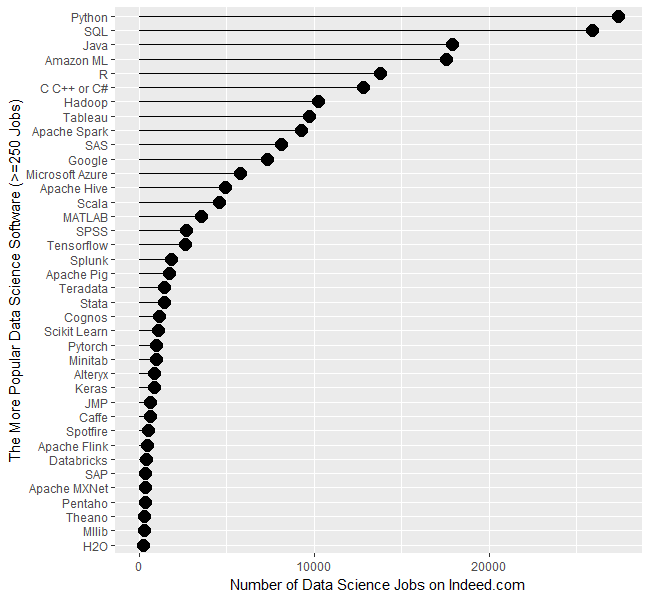
\includegraphics[width =
  0.53\textwidth]{pictures/number_of_data_science_jobs}
  \smallskip
  \fignote{\emph{Source} \url{http://r4stats.com/articles/popularity/}}

\end{figure}


\section{Basic setup}
\begin{itemize}
\item Download and install R from the R-project website
  \url{https://www.r-project.org/about.html}


  \item Download and install the free version of RStudio
    \url{https://rstudio.com/products/rstudio/download/}

      Please follow the defaults unless you have a good reason not to.
\end{itemize}

\section{Outline of guide/getting started}

\section{Additional resources}


\end{document}


%%% Local Variables:
%%% mode: latex
%%% TeX-master: t
%%% End:
